\section{Ion Beam Analysis}
\textbf{a)} To identify the unkown elemental compostitions of the film, substrate and beam, the \textit{Potku} \cite{potku}. By plotting the Energy as a function of Time-of-Flight (ToF), several elemental traces are visually apparent. It is possible to add 2D gates to delimit the edges of the traces in \textit{Potku}. The program can then perform a calibration if the gates and beam are labeled correctly. 

For this, a preliminary analysis of the shape of the plot has to be done. A hypothesis of the compositions can be developed from that. If the hypothesis is correct, the calibration will be linear and all point will lie on the calibration line. 

For the initial hypothesis, the strongest traces can be identified as the film. Since the only possible film compositions are \ce{Al_2O_3} and \ce{AlN}, we know that the more massive of these traces has to correspond to aluminium. By knowing that more massive atoms have a longer ToF, we can identify the strong trace on the right (the trace that has the highest energies) as the aluminium trace. All traces to the left of this one correspond to atoms which are lighter than it. 

There is only one trace to the right of this one, and the bottom of the trace is thicker, which indicates that there is an unresolved second trace next to it. Since a substrate candidate is silicon, the neighbouring element to aluminium, we can take it for the preliminary hypothesis, ruling out germanium. 

There is still a heavier atom than aluminium and silicon in the spectrum, so fluorine can be ruled out as a beam component. Due to the energy ratio between the last trace and the aluminium-tagged trace, we can take the heaviest possible beam component, Cu, for the hypothesis.

Finally, the traces to the left of the aluminium-tagged one have to be identified. Due to the structure seen, and knowing that the only candidates for these are nitrogen and oxygen as part of the film, the three-trace structure reveals that this must be nitrogen with some carbon and oxygen contamination. If the central, strong trace were oxygen, the slightly higher mass trace would have to be fluorine or neon contamination, which is unlikely. It is possible to see a faint trace just to the right of the strongest trace in that region. If the second element in the film is indeed nitrogen, this might be \ce{^{15}N}, a stable isotope of N with a natural abundance of 0.4\%. It can be present in nitrogen samples, but it will be almost negligible in comparison to \ce{^{14}N}.

Therefore, the discussed traces are identified as such in \textit{Potku}, with the areas shown in \autoref{fig:tof} as discussed. The resulting calibration plot is shown in \autoref{fig:calib}. It can be seen in this figure that the calibration points shown for the hyposethised atoms with Cu as a beam lie on the calibration line. It can therefore be confirmed that they were correctly selected. The time of flight calibration was as follows:
\begin{equation}
    \label{eq:tofcal}
    TOF[s] = 2.9941\E{-9}\unit{s} + TOF[Ch]\times5.5470\E{-11}\unit{s/Ch}
\end{equation}
\newpage

\begin{figure}[h!]
    \centering
    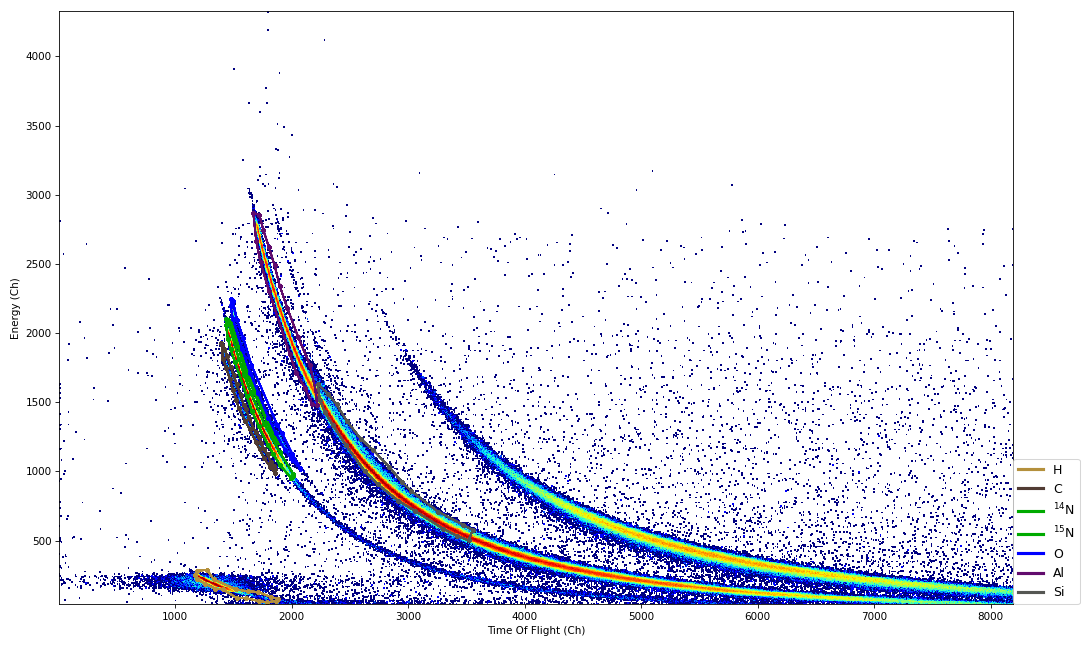
\includegraphics[width=1\textwidth]{ToF-E.png}
    \caption{Energy to Time of Flight diagram for the whole dataset, including gates for several elemental traces.}
    \label{fig:tof}
\end{figure}

\begin{figure}[h!]
    \centering
    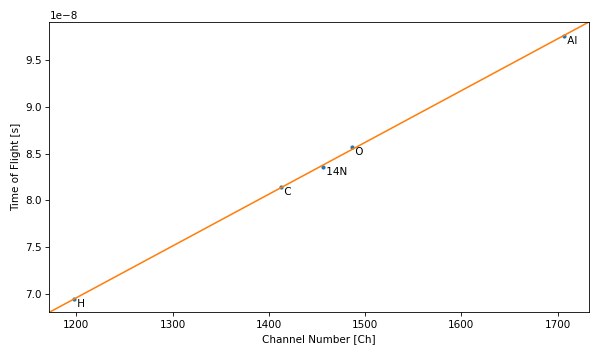
\includegraphics[width=\textwidth]{ToF-E_Calibration.png}
    \caption{Linear calibration performed by Potku, all points being on the line indicate that the elemental traces were tagged correctly.}
    \label{fig:calib}
\end{figure}
\newpage


The setup is, therefore, as follows: \begin{itemize}
    \item Beam: \ce{^{63}Cu},
    \item Substrate: \ce{{Si}},
    \item Foil: \ce{AlN}. 
\end{itemize}
In terms of impurities, there exists hydrogen, oxygen and carbon that don't originate from the beam, substrate or film. Therefore, they must be impurities. Hydrogen and oxygen are likely to come from water contamination (from the atmosphere). The carbon impurities may come from the Mylar foil used before the detector. This can also be an additional source of oxygen and hydrogen, as Mylar is made of these three elements.

The fourth impurity, close to the mass of aluminium, is barely visible, but it must be chlorine, in very low concentrations, as the precursor of the film was \ce{AlCl_3}. Some trace amounts of chlorine may still be present in the foil. This can be confirmed from the energy ratio of the faint chlorine trace and the aluminium trace.

\textbf{b)} As discussed in the previous section, the beam ion is \ce{^{63}Cu} and the subtrate is \ce{Si}. The beam's energy ratio to the other confirmed elements can only match that of copper, due to the other possibilities being much closer to aluminium, the strongest trace in the spectrum. The substrate could only be Si or Ge, and considering the widening of the aluminium trace towards the bottom, it can be seen that an adjacent element must be present in the sample. 

\textbf{c)} An energy calibration can be performed for the spectrum using the higher energy points of each respective trace and knowing that they will correspond to the case of surface extraction. Therefore, since there was no loss of energy in the film for those, the following equation is valid for their energy:
\begin{equation}
    E_R = \left(\frac{4M_IM_R \cos^2(\varphi)}{(M_I+M_R)^2}\right)E_I \equiv \Lambda_R E_I,
\end{equation} where an index $I$ represents the beam parameters and an index $R$ represents the detected recoil. $\varphi$ is the angle that the beam and detector make, in this case it will be 180$\deg$ - 41$\deg$, due to the geometry of the setup. Since the angle is constant and the beam composition does not change, the $\Lambda$ coefficient will be a constant for each of element in the problem, thus allowing for the estimation of their maximum energy and thus a calibration of the energy axis.

The maximum energies for the two elements in the foil, Al and N are: 
\begin{align}
    \label{eq:Emax}
    E_{\ce{N}}  (\text{surf}) = 4.033\unit{MeV}\\
    E_{\ce{Al}} (\text{surf}) = 5.694\unit{MeV}
\end{align}

With these, and estimating the maximum energy for each of their respective traces, with the maximum energy for N at 2100\unit{Ch} and the maximum energy for Al at 2825\unit{Ch}, a very rough linear calibration can be performed to the energy axis. This was:
\begin{equation}
    \label{eq:Ecal}
    E[MeV] = -0.778\unit{Ch} + E[Ch]\times0.0023\unit{Ch/MeV}.
\end{equation}

With this, it is possible to extract the minimum energy of \ce{^{14}N} (since that of Al is not resolvable due to the overlap with Si), as the bottom edge of the \ce{^{14}N} trace. As this is taken to be at energy channel 1934, the minimum energy of the \ce{^{14}N} recoils is taken as 3.670\unit{MeV}. This is the energy with which the \ce{^{14}N} recoils exit after having been emitted at 4.033\unit{MeV} and deposited $\Delta E = 0.363\unit{MeV}$ in a thickness $\tau$ of film. This $\tau$ will be the total thickness of the film. 

Using the stopping power of \ce{^{14}N} at 4.033\unit{MeV} in a sheet of \ce{AlN}, taken from SRIM \cite{srim}: $$\frac{\d E}{\d x} = 2.227\E{2}\unit{eV/(10$^{15}$\,at/cm$^2$)}$$ it is possible to estimate the thickness of the film as:
\begin{equation}
    \label{eq:film}
    T = \frac{\Delta E}{\left(\frac{\d E}{\d x}\right)} = \frac{363000\unit{eV}}{2.227\E{2}\unit{eV/(10$^{15}$\,at/cm$^2$)}} \approx 1629\E{15}\unit{at/cm$^2$} = 1.6\E{18}\unit{at/cm$^2$}.
\end{equation}

This, however is an overestimation, since the beam traverses a longer path from the end of the film to the surface, due to being emitted at a 20.5$\deg$ angle with respect to the normal of the film surface. Due to this, the true thickness of the sheet will be the result of \autoref{eq:film} multiplied by the cosine of this exit angle:
\begin{equation}
    \label{eq:filmcos}
    \boxed{\tau = T\cos(20.5\deg) = 1.5\E{18}\unit{at/cm$^2$}}.
\end{equation}
This is just an estimate, since there are several sources of uncertainty in the calculation. Firstly, it is not trivial to obtain the maximum and minimum energy points from the plot. Secondly, the energy calibration assumes linearity, which is also not possible to prove. The calibration is only performed with two points, which also introduces uncertainty. Addtionally, the energy loss should be calculated by an integration along the thickness of the film, instead of assuming a constant value. This is done because SRIM cannot provide with a smooth, integrable, function for the stopping power. 

\textbf{d)} A composition changes plot was extracted from \textit{Potku} and shown in \autoref{fig:composition}. In the figure, it can be seen that the components of the film vary with time in an oscillatory manner. The origin of this oscillation can be due to fluctuations in the beam. It can be seen in \autoref{fig:composition} that the oscillations in both of the film components is synchronised with the beam fluctuations. Therefore, we cannot observe any significant composition changes in the course of this experiment.

\begin{figure}[h!]
    \centering
    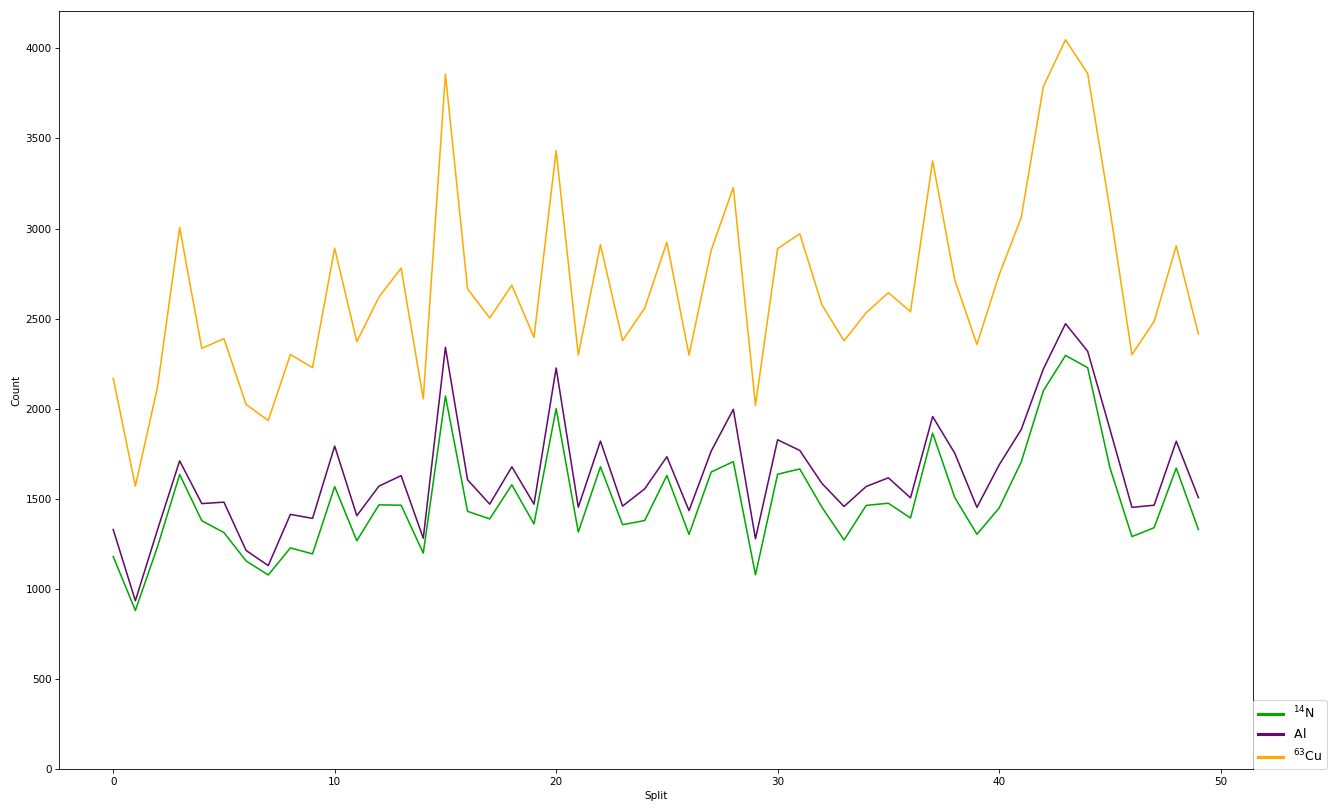
\includegraphics[width=\textwidth]{composition.png}
    \caption{Composition changes plot using \textit{Potku}. Aluminium (purple) and nitrogen (green) are plotted as the main components od the film. The copper beam (orange) is also plotted as a reference of beam behaviour.}
    \label{fig:composition}
\end{figure}
\newpage


\textbf{e)} In this case, Particle Induced X-ray Emission (PIXE) is not an optimal method to analyse the film and substrate, as it is in practice limited to elements with an atomic number higher than 13 (corresponding to Al). Since one of the foil components is N (Z = 7), this will not be seen using the PIXE technique. Additionally, the PIXE technique does not provide depth information of the sample, so this analysis would not be possible.

Nuclear Reaction Analysis (NRA) is generally better suited for lighter elements, approximately up to Mg. Al, one of the main components of the film, would already be in the limit of this technique. Also, in terms of depth information, NRA is somewhat limited in comparison to the TOF-ERDA method. There are also sometimes radiation safety concerns when using the NRA method, which may also be a reason to use other methods.

Rutherford Back-Scattering (RBS) may be used for analysis of samples like this one. However, RBS sometimes struggles with crystalline structures due to ion channeling. \ce{AlN} is a crystalline compound, so this may cause some difficulties when using the RBS method when compared to the TOF-ERDA technique.



